% Running head would be 68.9 pt too wide with the full title; the chapter page and
% the table of contents keep the complete title.
\judulpendek{Differential Privacy and QML}
\chapter{Differential Privacy and the Mathematical Foundations of QML}

A dental clinic collects the records of ten thousand patients, trains a model to
predict who is at high risk, and then publishes that model as a file of weights. The
following month a student takes one name from the patient list that leaked through
another channel, feeds that person's medical record into the model, and reads the
output score. The score is far higher than the scores of other people with similar
medical records who are not patients of that clinic. The student did not break into
the database and did not use anyone's password. He only asked the model, again and
again, and the model answered too confidently for someone it had seen during training.

A parallel to that incident sits at the other end of this book. A paper reports
``quantum advantage'' because its circuit prepares a state with $2^{50}$ amplitudes,
a number that no computer can store. The number is correct. What the paper does not
say: the amplitudes cannot be read, and the measurement result is only a sample.

The two stories have a defect of the same shape: the claim runs faster than the
mathematics that supports it. The first half of the chapter builds the definition
that makes the sentence ``this model is private'' testable, namely \emph{differential
privacy}, and then shows why that definition takes the form of a comparison of two
worlds rather than a prohibition on remembering. The second half builds the foundation
for assessing the sentence ``quantum models are superior'': complex amplitudes,
unitary gates, the Born rule, and the cost of simulation.

\index{differential privacy}
\index{quantum advantage}

\kamus{differential privacy}{privasi diferensial}{a promise that the result of a
procedure barely changes, in the sense of probability, when one person enters or leaves
the training data}

\begin{untukanak}
Imagine an ice cream shop that records the average amount spent by all customers that
day, and then sticks that number on the door. If Sari is the only customer who bought a
large birthday cake, the average that is posted goes up too, and a neighbor who knows
that it is Sari's birthday can guess that Sari is on that day's list of customers. The
number is not a name, but the number still tells a story about one person.

Now imagine a more careful shop. Before posting the number, it adds a small random
jitter, say thirty cents up or down, with equal probability. Whether Sari is included or
not, the number that is posted is nearly the same, because the jitter is much larger
than the influence of one person. Other customers can still learn that day's average
spending accurately enough, but there is no longer any way to determine whether Sari is
on the list.

The question that makes one curious: if the jitter is too small, the secret leaks; if
it is too large, the number is useless. Where is the honest boundary between them, and
how can we prove that the boundary is right? In this chapter we will learn why a privacy
promise has to take the form of a comparison of two nearly identical worlds, and not a
promise that the computer will forget.
\end{untukanak}

\section{What leaks from a model trained on personal data}
\tingkat{basic}

A model does not store a copy of the training data. It stores parameters, and those
parameters are chosen so as to fit the data. Precisely because of that choice the data
leave a trace, and the trace can be read in three ways of different difficulty.

The first way, \emph{membership inference}. The attacker has one medical record and
wants to know whether that record is in the training data. He does not need to open the
model; it is enough to send the record and read the output. A model trained on that
record usually answers with higher confidence, because the parameters have already been
adjusted to include it. Shokri, Stronati, Song, and Shmatikov showed in 2017 that this
difference in confidence is enough to be separated by a second classifier trained on
``shadow models'', namely copies of the model trained on data with and without a
particular example. The attack works on a model that can only be queried, with no
weights and no gradients.

The second way, \emph{attribute inference}. The attacker does not ask about membership,
but about a property that is not in the data: whether this person smokes, whether she is
pregnant. A model trained on a particular population can reveal correlations that should
not be used to decide anything about one person.

The third way, \emph{reconstruction}: the attacker recovers part of the contents of the
data. Dinur and Nissim showed in 2003 that a sequence of aggregate queries with small
noise still leaks most of the contents of a database when the queries are numerous and
interdependent. Zhu, Liu, and Han showed in 2019 that gradients in distributed training
can be used to recover training images almost exactly.

Those three channels explain why the sentence ``we publish only parameters, not data''
is not enough. What has to be promised is not ``nothing was copied'', but ``the output of
this procedure barely depends on one person''. To state that mathematically we need two
definitions of distance: the distance between two datasets that differ in one person,
and the distance between two output distributions.

\begin{definisi}[Neighboring datasets]
Two datasets $D$ and $D'$ over the same domain are called \emph{neighboring} when the
two are identical except in one record: $D'$ is obtained from $D$ by adding or removing
one record, or by replacing one record with another. The set of all such pairs is written
$\mathcal{N}$.
\end{definisi}

\index{membership inference}
The choice ``add or remove'' is called unbounded adjacency, ``replace'' is called bounded
adjacency, and the two give different sensitivity numbers. A privacy claim that does not
state the choice is incomplete.

\section{The definition of differential privacy, and why not an average}
\tingkat{intermediate}

``Nearly the same'' is measured with a ratio of probabilities, not with a difference,
because the ratio does not change when the probabilities are very small, and it is
precisely very small probabilities that attackers most often use to infer something.

\begin{definisi}[$(\varepsilon,\delta)$ differential privacy]
\index{differential privacy}
Let $\varepsilon\ge 0$ and $\delta\in[0,1]$. A randomized procedure $M$ that maps
datasets to an output space $\mathcal{Y}$ satisfies $(\varepsilon,\delta)$ differential
privacy when for every neighboring pair $(D,D')\in\mathcal{N}$ and every measurable set
$S\subseteq\mathcal{Y}$ we have
\begin{equation}
P\bigl[M(D)\in S\bigr] \;\le\; e^{\varepsilon}\,P\bigl[M(D')\in S\bigr] + \delta .
\end{equation}
If $\delta=0$, the procedure satisfies pure $\varepsilon$ differential privacy.
\end{definisi}

\begin{figure}[htbp]
\centering
\begin{tikzpicture}
\begin{axis}[width=6.2cm,height=4.1cm,xmin=-2.6,xmax=3.6,ymin=0,ymax=4.6,
  domain=-2.6:3.6,samples=200,axis lines=left,
  xtick={-2,-1,0,1,2,3},ytick={0,2,4},
  tick label style={font=\scriptsize},label style={font=\scriptsize},
  title={$\varepsilon=8$},title style={font=\scriptsize},
  xlabel={output},ylabel={density},
  legend style={font=\scriptsize,draw=none,at={(0.03,0.97)},anchor=north west},
  legend cell align=left]
  \addplot[thick,accent,fill=accent!12] {4*exp(-8*abs(x))} \closedcycle;
  \addlegendentry{data $D$}
  \addplot[thick,layerteal,densely dashed] {4*exp(-8*abs(x-1))};
  \addlegendentry{data $D'$}
\end{axis}
\end{tikzpicture}
\hfill
\begin{tikzpicture}
\begin{axis}[width=6.2cm,height=4.1cm,xmin=-2.6,xmax=3.6,ymin=0,ymax=0.142,
  domain=-2.6:3.6,samples=200,axis lines=left,
  xtick={-2,-1,0,1,2,3},ytick={0,0.05,0.1},yticklabels={$0$,$0.05$,$0.1$},
  tick label style={font=\scriptsize},label style={font=\scriptsize},
  title={$\varepsilon=0.25$},title style={font=\scriptsize},
  xlabel={output},
  legend style={font=\scriptsize,draw=none,at={(0.03,0.97)},anchor=north west},
  legend cell align=left]
  \addplot[thick,accent,fill=accent!12] {0.125*exp(-0.25*abs(x))} \closedcycle;
  \addlegendentry{data $D$}
  \addplot[thick,layerteal,densely dashed] {0.125*exp(-0.25*abs(x-1))};
  \addlegendentry{data $D'$}
\end{axis}
\end{tikzpicture}
\caption{The output distribution of the Laplace mechanism at sensitivity $1$ for two
neighboring databases that differ in one record, with a different vertical scale in the
two panels. At $\varepsilon=8$ the two curves are far apart, so one output is already
enough to guess which data were used. At $\varepsilon=0.25$ the two almost coincide: the
ratio of their ordinates at every point is at most $e^{0.25}\approx1.284$, so one output
hardly favors either dataset.}
\label{fig:dua-sebaran}
\end{figure}

A new reader usually asks two things: why a comparison of probabilities rather than an
average, and why there is a $\delta$ at all if $\varepsilon$ already measures the
leakage.

The answer to the first question is the core of the first half of the chapter. Note the
order of the quantifiers: \emph{for every} $S$, \emph{for every} neighboring pair. That
promise has to hold for any test $S$, including a test that the attacker picks after
seeing the mechanism. A definition in the form of an average puts the quantifier inside:
``there is a small expectation''. The two forms are not equivalent;
Figure~\ref{fig:dua-sebaran} shows the difference at two values of $\varepsilon$.

\begin{proposisi}
Let $M$ satisfy $(\varepsilon,0)$ differential privacy. Then for every attacker
algorithm $A$ whose output is only $0$ or $1$, and every neighboring pair $(D,D')$,
\begin{equation}
P\bigl[A\bigl(M(D)\bigr)=1\bigr] \;\le\; e^{\varepsilon}\,
P\bigl[A\bigl(M(D')\bigr)=1\bigr] .
\end{equation}
\end{proposisi}

\begin{proof}
The set $\{y : A(y)=1\}$ is measurable, so it may be used as $S$ in the definition.
Direct substitution gives the result.
\end{proof}

That proposition looks trivial, and its use is precisely to close the door that is often
used to defend a weak mechanism. If the promise holds only for the \emph{average} output,
an attacker can average the results of many repetitions so that the random components
cancel one another and what remains is a signal about one person. With a per-event
promise, every repetition pays its own privacy budget.

\begin{bacakeras}
Read alternately, two voices. The first voice asks, the second voice answers.

``If one person leaves the list, does your answer change?''\\
``Slightly.''\\
``How slightly?''\\
``Slightly enough that nobody can be certain.''

Repeat that conversation three times, faster and faster, until it feels like a
recitation. Then the first voice asks again, more slowly:

``If I repeat that question a hundred times, is a hundred times slight still slight?''

Stay silent for one breath. Answer together: something slight repeated a hundred times
is no longer slight. Then say together, once: one person must not be able to change the
conclusion. Repeat that line once more, more slowly, and then once again while pointing
at one empty chair in the room.
\end{bacakeras}

\begin{contoh}[Randomized response]
\index{randomized response}
A respondent is asked whether he has ever used an illegal drug. The procedure: toss a
coin; if side A comes up, answer honestly; if side B comes up, toss again and answer
``yes'' if heads, ``no'' if tails. The probability of answering ``yes'' if he really uses
the drug is $1/2+1/2\cdot 1/2=3/4$, and if he does not use it the probability is
$1/2\cdot 1/2=1/4$. The ratio of the two is $3$, so $\varepsilon=\ln 3=1.0986$. No answer
proves anything about one person, and that is what the definition promises.
\end{contoh}

\begin{tangan}
Materials: one coin per person, paper, pencil. Ten friends each write one yes/no secret
on a slip of paper and fold it.

The rule is one. Toss the coin: heads, answer honestly; tails, toss again, heads means
``yes'' and tails means ``no''. Each person says only one word, and the recorder writes
only two groups of tally marks.

Now ask one person to change his secret, then repeat the whole round. Look at the tally
marks: they shift by at most one, and nobody can point to anyone. Conclusions about the
group survive. A conclusion about one person never appears.
\end{tangan}

Now $\delta$, namely the failure probability: with probability at most $\delta$ the ratio
promise may be violated entirely. Hence $\delta$ is not a tolerance that can be chosen at
will. If $\delta$ is comparable to $1/n$ for $n$ records, an attacker can target one
person and let the rest serve as camouflage; that is why $\delta$ must be much smaller
than $1/n$. The number $\varepsilon$ is not a probability either: $\varepsilon=1$ means a
probability ratio of at most $e\approx 2.718$, whereas $\varepsilon=8$ means a ratio up to
$2\,981$.

\section{Global sensitivity and the Laplace mechanism}
\tingkat{intermediate}

The only thing that stops us from adding noise arbitrarily is the question: how far can
one record shift the answer?

\begin{definisi}[Global sensitivity]
\index{global sensitivity}
For $f$ that maps datasets to $\mathbb{R}^d$, its global sensitivity is
\begin{equation}
\Delta f \;=\; \sup_{D\sim D'} \bigl\| f(D)-f(D') \bigr\|_{1},
\end{equation}
with the supremum taken over all neighboring pairs.
\end{definisi}

A count query, $f(D)=|D|$, has $\Delta f=1$. A sum query over values in $[0,R]$ has
$\Delta f=R$. An average query over $n$ records has $\Delta f=R/n$, because one person
shifts the average by only $R/n$; here it becomes visible that an average is safer than a
sum, but only as long as $n$ is known and fixed. Sensitivity also depends on the choice
of adjacency: if $D'$ may replace, the count query has $\Delta f=2$.

\begin{teorema}[Laplace mechanism]
\index{Laplace mechanism}
Let $f$ have global sensitivity $\Delta f$, and let $Y$ be distributed according to a
Laplace distribution with scale $b=\Delta f/\varepsilon$, that is with density
$p_b(y)=\frac{1}{2b}e^{-|y|/b}$. Then $M(D)=f(D)+Y$ satisfies $(\varepsilon,0)$
differential privacy.
\end{teorema}

\begin{proof}
Take $S\subseteq\mathbb{R}$ measurable and $D\sim D'$. It is enough to show that for
every $y$,
\begin{equation}
\frac{p_b\bigl(y-f(D)\bigr)}{p_b\bigl(y-f(D')\bigr)} \;\le\; e^{\varepsilon}.
\end{equation}
With $a=f(D)$ and $a'=f(D')$, the left-hand side is $\exp\bigl((|y-a'|-|y-a|)/b\bigr)$.
The triangle inequality gives $|y-a'|-|y-a|\le|a-a'|$, so the left-hand side is at most
$\exp(|a-a'|/b)\le\exp(\Delta f/b)=e^{\varepsilon}$, because $\Delta f$ is the supremum.
Hence $p_b(y-a)\le e^{\varepsilon}p_b(y-a')$ for every $y$; integrating both sides over
$S$ gives $P[M(D)\in S]\le e^{\varepsilon}P[M(D')\in S]$, and because there is no
remainder term, $\delta=0$.
\end{proof}

A numerical example goes like this. For a count query with $\varepsilon=0.5$, the scale
is $b=1/0.5=2$; the probability that the noise exceeds $5$ in absolute value is
$e^{-5/2}=0.0821$, so about one answer in twelve misses by more than five people.
Conversely, with probability $0.95$ the error does not exceed
$b\ln 20=2\times 2.9957=5.991$. Here the trade-off that recurs throughout the chapter
becomes visible: shrinking $\varepsilon$ enlarges $b$, and enlarging $b$ worsens
precision linearly.

\begin{resep}
\begin{enumerate}
  \item Fix $f$ and clip every value to the range $[0,R]$ before anything is computed.
  \item Compute $\Delta f$ from the worst case of one record on the clipped data.
  \item Choose $\varepsilon>0$, compute $b=\Delta f/\varepsilon$, add Laplace noise of
        scale $b$ to the answer.
  \item Record $\varepsilon$ in the budget book; the remaining budget is what has not
        been spent.
\end{enumerate}
A warning about order: clipping after the noise has been added changes the output
distribution and cancels the guarantee, because $\Delta f$ was computed from the data
before clipping.
\end{resep}

\kamus{global sensitivity}{sensitivitas global}{how far one person can shift the answer
of a query in the worst case; this is what determines the amount of noise that is needed}

Sometimes Laplace noise does not fit, for instance because the output is
high-dimensional. There Gaussian noise is used: for $f$ with $\ell_2$ sensitivity
$\Delta_2 f$, the mechanism $M(D)=f(D)+N(0,\sigma^{2}\Delta_2 f^{2}I)$ satisfies
$(\varepsilon,\delta)$ when $\sigma\ge\sqrt{2\ln(1.25/\delta)}/\varepsilon$. The proof is
skipped here; it compares two shifted normals with a concentration inequality, and the
full version is in Dwork and Roth (2014), appendix A. That condition is sufficient, not
necessary: for small $\sigma$ it is far looser than the true bound, and the tight bound
is given by the analytic Gaussian mechanism of Balle and Wang (2018).

\section{Composition: the privacy budget and why it runs out}
\tingkat{advanced}

A single mechanism is rarely used once. A model is trained with hundreds of steps, each
leaking a little, and what is needed is the total.

\begin{teorema}[Basic composition]
\index{composition}
Let $M_1,\dots,M_T$ be chosen adaptively, that is $M_t$ may depend on the outputs
$M_1,\dots,M_{t-1}$, and let every $M_t$ satisfy $(\varepsilon_t,\delta_t)$ for all
possible inputs. Then the joint output $(M_1,\dots,M_T)$ satisfies
$\bigl(\sum_t\varepsilon_t,\sum_t\delta_t\bigr)$.
\end{teorema}

\begin{proof}
It is enough to take $T=2$; the rest is induction. By the law of total probability,
\begin{align}
P\bigl[(M_1,M_2)\in S_1\times S_2\bigr]
&= \int_{S_1} P\bigl[M_1(D)\in dy_1\bigr]\,
   P\bigl[M_2(D,y_1)\in S_2 \mid M_1(D)=y_1\bigr] \notag\\
&\le \int_{S_1} e^{\varepsilon_1}P\bigl[M_1(D')\in dy_1\bigr]\,
   \bigl(e^{\varepsilon_2}P[M_2(D',y_1)\in S_2]+\delta_2\bigr) + \delta_1 \notag\\
&\le e^{\varepsilon_1+\varepsilon_2}P\bigl[(M_1,M_2)(D')\in S_1\times S_2\bigr]
   + \delta_1 + \delta_2 .
\end{align}
The first step uses the guarantee for $M_2$ at fixed $y_1$, the second step uses the
guarantee for $M_1$ and $P[M_1(D')\in S_1]\le 1$.
\end{proof}

Basic composition adds up, and that addition is what makes the budget run out quickly: a
hundred steps with $\varepsilon=0.1$ per step already spend $\varepsilon=10$. There is a
sharper bound when the leakage per step is small.

\begin{tantangan}
An office publishes the average salary of its team with Laplace noise of scale
$b=\Delta f/\varepsilon$, with $\varepsilon=1$ and $\Delta f=1$. It says, ``one answer
already satisfies $\varepsilon=1$, so one person is safe.'' How many times may that
answer be published before the average of those answers is sharp enough to guess the
salary of one person, and why?

Hint 1: random noise has mean zero; watch what happens to the average of the noise when
the answer is repeated.

Hint 2: the standard error of the average of $k$ answers is $b\sqrt{2}/\sqrt{k}$. With
$b=1$ and $k=100$ its value is $0.1414$, whereas one person can shift the answer by $1$.

If you get stuck, go back to the section on Composition.
\end{tantangan}

\begin{teorema}[Advanced composition]
For every $\varepsilon'>0$, the composition of $T$ procedures that each satisfy
$(\varepsilon,\delta)$ satisfies $(\varepsilon_{\mathrm{tot}},\delta_{\mathrm{tot}})$
with
\begin{equation}
\varepsilon_{\mathrm{tot}} = \sqrt{2T\ln(1/\delta')}\;\varepsilon
+ T\,\varepsilon\bigl(e^{\varepsilon}-1\bigr),
\qquad
\delta_{\mathrm{tot}} = T\delta + \delta' .
\end{equation}
\end{teorema}

The proof is skipped: it is obtained by bounding the moments of the probability ratio, or
with a moments \emph{accountant}. The references are Dwork and Roth section 3.5, and
Kairouz, Oh, and Viswanath (2015) for optimal composition. Its first term grows like
$\sqrt{T}$, not like $T$.

However, advanced composition is not always better, and this is often misquoted. The
second term, $T\varepsilon(e^{\varepsilon}-1)$, blows up when $\varepsilon$ is not small.
In the experiment in section eleven, with $T=200$ and $\delta=10^{-5}$, basic composition
gives $\varepsilon=36.5$ at $\sigma=32$ whereas advanced composition gives $20.6$; at
$\sigma=2$ the two give $583.7$ and $11\,302.8$. So advanced composition wins when
$\varepsilon$ per step is small and loses when it is large.

One more result makes the budget go further: when several procedures work on disjoint
parts of the data, their leakage is not added but the largest is taken, because one
record is in only one part. Splitting the data among several users, each with its own
budget, is far more economical than one user who runs all the queries.

\index{privacy budget}

\section{DP-SGD: clip, add noise, and the price that is paid}
\tingkat{advanced}

Ordinary training satisfies no definition at all, because one example can shift the
gradient by any amount: there is no upper bound on $\Delta f$, so the noise that is
needed is infinite. The repair consists of two steps that support each other.

The first step, clipping: every per-example gradient is clipped so that its norm does not
exceed $C$,
\begin{equation}
\operatorname{clip}_C(g) \;=\; g\cdot\min\Bigl(1,\;\frac{C}{\|g\|_2}\Bigr).
\end{equation}
After clipping, one example contributes at most $C$ to the sum, so the sensitivity of the
average over a batch of size $B$ is $C/B$. The second step, Gaussian noise with standard
deviation $\sigma C/B$ is added to that average,
\begin{equation}
w_{t+1} = w_t - \eta\Bigl(\frac{1}{B}\sum_{i\in\mathcal{B}_t}
\operatorname{clip}_C\bigl(\nabla\ell_i(w_t)\bigr) + \frac{\sigma C}{B}\,\xi_t\Bigr),
\qquad \xi_t\sim N(0,I).
\end{equation}
This algorithm is what is called DP-SGD, introduced by Abadi and colleagues in 2016
together with the moments \emph{accountant} that makes its budget computable for hundreds
of thousands of steps.

\begin{teorema}
Every DP-SGD step satisfies $(\varepsilon_0,\delta)$ with
\begin{equation}
\varepsilon_0=\sqrt{2\ln(1.25/\delta)}\,\big/\,\sigma ,
\end{equation}
and after $T$ steps the whole procedure satisfies $(T\varepsilon_0,T\delta)$.
\end{teorema}

\begin{proof}
The $\ell_2$ sensitivity of the average of clipped gradients is $C/B$, because replacing
one example shifts the average by at most $C/B$. Apply the Gaussian mechanism from
section three, then basic composition from section four.
\end{proof}

\index{dp-sgd}
The numbers from our experiment explain why the noise does not immediately erase the
learning. With $n=200$, $C=1$, and $\sigma=32$, the standard deviation of the noise per
coordinate is $32/200=0.16$, whereas the norm of the average gradient at the starting
point is $0.83$: the noise is about one fifth of the signal. But the noise changes sign
at random, so its contribution to the final position grows like $\sqrt{T}$, whereas the
signal grows like $T$. After two hundred steps the signal wins, and the model still
reaches $93.71$ percent.

What has to be paid is also visible. At $\sigma=128$ the accuracy falls to $85.51$
percent with a spread of $6.16$ across seeds; at $\sigma=512$ the accuracy is $70.39$
percent with a spread of $17.26$. That growing spread is not an oddity: at large noise
the result of training depends on the noise draws that happen to occur, so a single model
is no longer a sample that represents the procedure. Reporting one seed at large $\sigma$
would be misleading.

Four limits have to be mentioned together with that result. First, clipping introduces
bias: examples with large gradients, usually the hard or rare ones, are clipped harder, so
the model pays them less attention. Second, DP-SGD demands more steps, and that
computational cost is real. Third, the privacy guarantee is uniform but its utility cost
is not: Bagdasaryan, Poursaeed, and Shmatikov showed in 2019 that minority groups can
suffer a much larger drop in accuracy at the same budget. Fourth, and most important:
differential privacy guarantees something about \emph{individuals}, not about the
\emph{truth of the model}. A model with $\varepsilon=0.1$ can still be completely wrong,
can still be discriminatory, and can still be used for unfair decisions. Privacy is a
promise about how much one person can be learned from the output; it is not in the least a
promise that the output is any good.

\kamus{privacy budget}{anggaran privasi}{the total amount of $\varepsilon$ that a system
may spend; every query or training step spends some of it, and once it is exhausted there
is no guarantee left}

\section{Why amplitudes use complex numbers}
\tingkat{basic}

Now the second half, starting from a question that is often taken as technical although
its answer is conceptual. Why is a quantum state represented by complex numbers, and not
by real numbers?

The short answer: because two paths to the same result have to be able to cancel each
other, and cancellation of that kind demands a sign that can rotate, not merely positive
and negative. With real numbers an amplitude has only two signs, and interference can
only add or subtract. With complex numbers an amplitude has a phase that rotates
continuously, so two paths can meet at any angle and the result varies smoothly.

The complex number $z=a+bi$ with $i^2=-1$ has modulus $|z|=\sqrt{a^2+b^2}$, conjugate
$\bar z=a-bi$, and phase $\theta$ in the notation
$z=|z|e^{i\theta}=|z|(\cos\theta+i\sin\theta)$. Modulus and phase play different roles and
cannot be exchanged: the modulus determines the size of the probability, the phase
determines the sign of the interference. Multiplying two complex numbers multiplies the
moduli and adds the phases, and that property makes the phase useful as a coordinate of
the state.

\kamus{probability amplitude}{amplitudo}{a complex number whose modulus squared is the
probability; different from a probability because amplitudes can cancel one another}

The state space of one qubit is $\mathbb{C}^2$, and the state space of $n$ qubits is
$\mathbb{C}^{2^n}$ with the inner product
$\langle\phi|\psi\rangle=\sum_k\overline{\phi_k}\psi_k$. In bra-ket notation,
$|\psi\rangle$ is a column vector and $\langle\psi|$ is its conjugate transpose. A state
is always normalized, $\langle\psi|\psi\rangle=1$, because the sum of all probabilities
has to be one.

\begin{definisi}[Finite-dimensional Hilbert space]
\index{Hilbert space}
A finite-dimensional Hilbert space is a finite-dimensional complex vector space equipped
with a complete inner product. In this book the only example that is used is
$\mathbb{C}^{d}$ with the standard inner product, usually $d=2^{n}$.
\end{definisi}

Two properties of this notation have to be held from the start. First, the global phase
has no physical meaning: $|\psi\rangle$ and $e^{i\theta}|\psi\rangle$ give the same
probability for every measurement outcome, because $|e^{i\theta}a_k|^2=|a_k|^2$. Second,
the \emph{relative} phase has full meaning: changing the phase of one component alone
changes the result of interference, and that is what quantum algorithms use. The
difference between the invisible global phase and the visible relative phase becomes
clear in the worked example in section nine.

\begin{proposisi}
If $|\psi\rangle$ and $|\phi\rangle$ are both of norm one, then
$|\langle\phi|\psi\rangle|\le 1$.
\end{proposisi}

\begin{proof}
The Cauchy-Schwarz inequality gives
$|\langle\phi|\psi\rangle|^2\le\langle\phi|\phi\rangle\langle\psi|\psi\rangle=1$, then
take the square root.
\end{proof}

\section{Gates as unitary matrices, and why they must be unitary}
\tingkat{intermediate}

A change of state due to a gate is a matrix multiplication,
$|\psi'\rangle=U|\psi\rangle$. Not every matrix may be used. The condition is one: the
total probability has to stay one for every initial state, so
$\langle U\psi|U\psi\rangle=\langle\psi|\psi\rangle$ for all $\psi$.

\begin{definisi}[Unitary matrix]
\index{unitary gate}
A square matrix $U$ is called unitary when $U^{\dagger}U=UU^{\dagger}=I$, with
$U^{\dagger}$ the conjugate transpose of $U$.
\end{definisi}

\begin{teorema}
For a square matrix $U$ over $\mathbb{C}^{d}$, the following statements are equivalent:
(i) $U$ is unitary; (ii) $\langle U\phi|U\psi\rangle=\langle\phi|\psi\rangle$ for all
$\phi,\psi$; (iii) $\|U\psi\|=\|\psi\|$ for all $\psi$.
\end{teorema}

\begin{proof}
(i) $\Rightarrow$ (ii): $\langle U\phi|U\psi\rangle=\phi^{\dagger}U^{\dagger}U\psi
=\phi^{\dagger}\psi$. (ii) $\Rightarrow$ (iii): take $\phi=\psi$. (iii)
$\Rightarrow$ (i): from $\langle U\psi|U\psi\rangle=\langle\psi|\psi\rangle$ for all
$\psi$, use the polarization identity to conclude
$\langle\phi|U^{\dagger}U\psi\rangle=\langle\phi|\psi\rangle$ for all $\phi,\psi$;
therefore $U^{\dagger}U=I$, and for a square matrix in finite dimension a left inverse
means a right inverse.
\end{proof}

That theorem explains three things. First, a gate must be unitary because probability must
be conserved; no other reason is needed. Second, every gate has an inverse $U^{\dagger}$
that is also unitary, so a circuit can be reversed and no information is lost while the
gates act. Third, the only non-unitary operation is measurement, and that is where
information is lost. That is why quantum computation is not computation that erases
information, but computation that postpones erasure until the end.

\begin{proposisi}[No cloning]
There is no unitary $U$ on two qubits such that
$U\bigl(|\psi\rangle\otimes|0\rangle\bigr)=|\psi\rangle\otimes|\psi\rangle$ for all
$|\psi\rangle$.
\end{proposisi}

\begin{proof}
Suppose there is one, and take $|\psi\rangle,|\phi\rangle$ of norm one. Because $U$ is
unitary, the inner products of the two sides are equal:
$\langle\phi|\psi\rangle=\langle\phi|\psi\rangle^2$. The equation $x=x^2$ has only the
solutions $0$ and $1$, so every pair of states has to be orthogonal or identical; that is
impossible for more than two states.
\end{proof}

\kamus{unitary}{uniter}{a property of a matrix that preserves the length of a vector; in
everyday language, a gate that neither adds nor removes total probability}

\section{Fourier as a change of basis, and its connection to convolution}
\tingkat{advanced}

The Fourier transform is a change of basis, and that is the most useful way to see it
here. In a space of dimension $N$, the standard basis is replaced by the basis
$|f_k\rangle$ whose components are $(|f_k\rangle)_j=\omega^{jk}/\sqrt{N}$ with
$\omega=e^{2\pi i/N}$. The matrix is $F_{jk}=\omega^{jk}/\sqrt{N}$.

\begin{proposisi}
The Fourier matrix $F$ is unitary.
\end{proposisi}

\begin{proof}
Compute $(F^{\dagger}F)_{jk}=\frac{1}{N}\sum_{l=0}^{N-1}\omega^{-lj}\omega^{lk}
=\frac{1}{N}\sum_{l=0}^{N-1}\omega^{l(k-j)}$. If $k=j$ every term has the value one, so
the result is $1$. If $k\neq j$, this is a geometric series with ratio
$\omega^{k-j}\neq1$ and its sum is $\frac{1-\omega^{N(k-j)}}{1-\omega^{k-j}}=0$ because
$\omega^{N}=1$. Hence $F^{\dagger}F=I$.
\end{proof}

Because it is unitary, $F$ may legitimately be used as a gate, and its $n$-qubit version
is called the quantum Fourier transform. What makes it interesting is not only that it is
a legitimate gate, but that it turns convolution into pointwise multiplication.

\begin{teorema}[Convolution becomes multiplication]
\index{convolution}
For $x,y\in\mathbb{C}^{N}$, define the cyclic convolution
$(x*y)_k=\sum_{j=0}^{N-1}x_j\,y_{(k-j)\bmod N}$. Then
\begin{equation}
F(x*y) \;=\; \sqrt{N}\,\bigl(Fx\bigr)\odot\bigl(Fy\bigr),
\end{equation}
with $\odot$ the componentwise product.
\end{teorema}

\begin{proof}
The $k$-th component of the left-hand side is
$\frac{1}{\sqrt{N}}\sum_m\omega^{km}\sum_j x_j y_{m-j}$. Exchange the order of summation
and write $r=m-j$:
\[
\frac{1}{\sqrt{N}}\sum_j x_j\omega^{kj}\sum_r\omega^{kr}y_r
=\sqrt{N}\,(Fx)_k\,(Fy)_k .
\]
The exchange of the order of summation is legitimate because both sums are finite.
\end{proof}

That exchange of two finite sums looks trivial, but the infinite version of the same step
is the content of Chapter 14: a Fourier series may be differentiated term by term only
when its convergence is uniform enough. The connection with Chapter 15 is more
conceptual: a change of basis is a change of variable, and a unitary matrix is a change of
variable whose Jacobian determinant has modulus one, so volumes and probabilities do not
change.

The connection with quantum computation lies in its cost. A discrete Fourier transform
over $N=2^{n}$ points is computed classically in $\mathcal{O}(N\log N)$ operations with
the FFT. Its quantum version is built from $\mathcal{O}(n^{2})$ gates. The difference is
real and is the basis of Shor's algorithm. But there is a condition that is often left
out: once the transform is finished, we cannot read the $N$ amplitudes, and all we can do
is take samples. Speed in preparing a state does not automatically become speed on the
task one wants to finish; it has to be paired with a procedure that extracts the answer
from only a few samples. Many claims of quantum advantage in machine learning have no
procedure of that kind.

\section{The Born rule, and why the output is always probabilistic}
\tingkat{intermediate}

Up to here everything is deterministic: given a state and a gate, the next state is
unique. Probability enters at one step that cannot be avoided, namely measurement.

\begin{definisi}[Born rule]
\index{Born rule}
If the state $|\psi\rangle=\sum_k a_k|k\rangle$ is measured in the orthonormal basis
$\{|k\rangle\}$, the probability of obtaining outcome $k$ is
\begin{equation}
p(k) \;=\; \bigl|\langle k|\psi\rangle\bigr|^{2} \;=\; |a_k|^{2},
\end{equation}
and after the outcome $k$ is obtained, the state becomes $|k\rangle$.
\end{definisi}

Why must it be so, and not merely our ignorance of the state that is ``really'' there?
The strongest answer is not philosophical but experimental: Bell's inequality, tested by
Aspect, Grangier, and Roger in 1982, shows that the correlations between two separated
measurements violate a bound that every theory storing hidden definite values has to obey.
So probabilism here is not a way of saying ``we do not know yet''; it is the structure of
the theory. The practical consequence: one measurement gives one outcome, not the whole
state.

\kamus{Born rule}{aturan Born}{the rule that turns an amplitude into a probability by
squaring its modulus; the only place where probability enters the theory}

The consequence for machine learning is often underestimated. To estimate $p(k)$ with
standard error $\gamma$ one needs about $p(1-p)/\gamma^{2}$ shots. In our experiment, the
state $R_y(60^\circ)|0\rangle$ has true probabilities $0.75$ and $0.25$; with a thousand
shots the recorded counts were $727$ and $273$, the estimate $0.727$, differing by
$0.023$ from the true value. Its theoretical standard error is
$\sqrt{0.75\cdot 0.25/1000}=0.0137$, so that difference is about $1.7$ standard errors, an
ordinary event. Three digits after the decimal point need about a million shots, and every
shot means one state preparation and one measurement. This is where the factor $\sqrt{N}$
appears, and this is where many ``quadratic speeds'' turn into ordinary speeds once the
cost of readout is counted.

\section{Worked example: one and two qubits by hand}
\tingkat{intermediate}

\begin{untukanak}
Two children toss coins. The first child tosses one coin, then closes his hand and asks:
heads or tails? The result is one, and nobody can know anything before that coin is
opened. The second child prepares two coins in a strange way: he tells the coins to
``consult'' first, so that the two always agree, without ever agreeing in advance whether
they will both be heads or both be tails. When the first coin is opened and shows heads,
the second coin is certainly heads. When the first coin shows tails, the second coin is
certainly tails.

What makes it strange: there is no way to make two ordinary coins behave like that. If
both were fixed from the start, whoever made the coins would know both. In coins that
consult there is no record of that kind, and real experiments show that no hidden record
explains the outcome.

That last example is what is called a Bell state, and this chapter uses it to show why
``zero'' and ``very small'' are two different things.
\end{untukanak}

All the numbers in this section are rechecked with NumPy in section eleven, and the reader
can check them with an ordinary calculator.

The Hadamard gate on one qubit is
$H=\frac{1}{\sqrt{2}}\begin{pmatrix}1&1\\1&-1\end{pmatrix}$. On $|0\rangle=(1,0)$ it gives
\[
H|0\rangle=\frac{1}{\sqrt{2}}(1,1)=(0.7071;\;0.7071),
\]
so the probabilities of the outcomes $0$ and $1$ are $0.5$ each.

Now the circuit $H$, then $Z=\operatorname{diag}(1,-1)$, then $H$ again. The first step
gives $(0.7071;0.7071)$; the second step flips the sign of the second component to
$(0.7071;-0.7071)$; the third step multiplies by $H$:
\[
H\begin{pmatrix}0.7071\\-0.7071\end{pmatrix}
=\frac{1}{2}\begin{pmatrix}0.7071-0.7071\\0.7071+0.7071\end{pmatrix}
=\begin{pmatrix}0\\1\end{pmatrix}.
\]
The result is $|1\rangle$ with probability one. The amplitude of the $|0\rangle$ component
becomes zero not because something was thrown away, but because two paths meet with
opposite signs. This is interference, and this is why the relative phase matters: if $Z$
is replaced by the identity, the result is $|0\rangle$ again.

The third example uses a rotation. The gate
$R_y(\theta)=\begin{pmatrix}\cos(\theta/2)&-\sin(\theta/2)\\
\sin(\theta/2)&\cos(\theta/2)\end{pmatrix}$ rotates the state in the real plane. With
$\theta=60^\circ$ and initial state $|0\rangle$,
\[
R_y(60^\circ)|0\rangle=(\cos 30^\circ;\;\sin 30^\circ)=(0.8660;\;0.5),
\]
so the probabilities are $\cos^{2}30^\circ=0.75$ and $\sin^{2}30^\circ=0.25$. Note that
$|a_0|^2+|a_1|^2=0.75+0.25=1$.

The fourth example is two qubits. Start from $|00\rangle$, apply $H$ to the first qubit,
then CNOT with the first qubit as control and the second as target. After $H$ the state is
$\frac{1}{\sqrt{2}}(|00\rangle+|10\rangle)$. CNOT flips the second qubit only when the
first qubit is $1$, so
\[
|\Phi^{+}\rangle=\frac{1}{\sqrt{2}}\bigl(|00\rangle+|11\rangle\bigr)
=(0.7071;\;0;\;0;\;0.7071).
\]
The probabilities of $00$ and $11$ are $0.5$ each; the probabilities of $01$ and $10$ are
zero. The two amplitudes in the middle are zero because the two paths that lead there
cancel one another, not because both are impossible. Consequently, if both qubits are
measured, the outcomes always agree: $00$ or $11$, never a mixture.

\kertas{Check the examples above without looking at the text. (a) Compute $HZH|0\rangle$
by writing out every matrix multiplication, then explain why the result is $|1\rangle$ and
not $|0\rangle$. (b) Replace $R_y(60^\circ)$ with $R_y(90^\circ)$, compute both
probabilities, then explain why two different states can give the same probabilities.
(c) For the Bell state above, compute the probability of obtaining $01$ and explain why
that number is zero, and not ``very small''.}

\section{Why classical simulation explodes, and what that means for claims of advantage}
\tingkat{advanced}

The state of $n$ qubits is a vector in $\mathbb{C}^{2^{n}}$, so it has $2^{n}$ complex
amplitudes. For $n=10$ that is $1\,024$ numbers, no larger than a small image. For $n=50$
it is $2^{50}=1.1259\times10^{15}$ numbers; with $16$ bytes per amplitude, what is needed
is $2^{54}$ bytes, that is exactly $16$ pebibytes. It is a limit that doubles every time
one qubit is added.

The experiment in section eleven measures the consequence. Preparing a state with one
Hadamard gate on every qubit takes $0.2$ milliseconds for $n=10$, $2.3$ for $n=14$, $81.4$
for $n=18$, and $1\,357$ milliseconds for $n=22$. That time column is the noisiest in the
whole chapter: two runs on the same machine can differ by almost a factor of two. What
does not change is the pattern, namely a straight line on a logarithmic scale against
$2^{n}$.

What may and may not be concluded? What may: a general quantum state cannot be stored
classically for large $n$, so an algorithm that genuinely uses all $2^{n}$ amplitudes
cannot be imitated directly. What may not: that every quantum circuit is faster. There are
three reasons.

The first reason, the state cannot be read. One measurement gives one outcome, whereas a
classical simulation that stores the whole vector can compute the probability of every
outcome. So more information is available in the simulation than in the hardware, and the
inability to copy a state is not evidence of advantage.

The second reason, the circuits that can be simulated include many circuits that are used
in practice: small depth, limited entanglement, product states, and Clifford gates have
efficient classical imitations. Goguen, Clarke, Martens, and Selman showed that family of
circuits can be computed classically in polynomial time, and that family is wide enough to
include many variational ansatzes.

The third reason, advantage can be removed by data structure. Ewin Tang showed in 2019
that a quantum recommendation algorithm that was thought to give an exponential speedup
has a classical counterpart with a polynomial speedup, because the structure of its data
matrix can be exploited without quantum mechanics. Huang, Kueng, and Preskill (2021) give
a strict separation, but only for a particular family of data distributions.

\kamus{barren plateau}{plateau tandus}{a region of the loss landscape of a variational
circuit where the gradients shrink exponentially in the number of qubits, so that
training does not move}

An honest statement about QML in 2026 therefore takes this form. There is evidence of
separation for particular tasks in oracle models, and there are theoretical claims of
speedup for learning tasks under particular distributional assumptions. There is no
established evidence of practical advantage for machine learning tasks on classical data,
in the sense of an experiment repeated on real hardware that beats the best classical
method at a meaningful data size. Cerezo and colleagues (2021, 2022) call the
\emph{barren plateau}, namely gradients that vanish exponentially in deep circuits, an
unresolved obstacle rather than a technical detail.

\section{Computational lab: privacy budget, accuracy, and the size of a state}
\tingkat{advanced}

The following program runs the two experiments above with no library other than NumPy:
DP-SGD on two-class logistic regression with five seeds per noise level, then several
quantum states and the cost of simulating them. All the numbers in this chapter come from
the output below, except those marked as hand computations.

\begin{lab}
\begin{verbatim}
import numpy as np
import time

D, N, T, C, DELTA, LR = 8, 200, 200, 1.0, 1e-5, 0.5


def data(rng, n, mu=0.6):
    y = 2 * rng.integers(0, 2, n) - 1
    return rng.normal(mu * y[:, None], 1.0, (n, D)), y


def sig(t):
    return 1.0 / (1.0 + np.exp(-t))


def clip(G):
    nrm = np.linalg.norm(G, axis=1, keepdims=True)
    return G * np.minimum(1.0, C / np.maximum(nrm, 1e-9))


def dp_sgd(X, y, sigma, seed):
    rng = np.random.default_rng(seed)
    w = np.zeros(D)
    for _ in range(T):
        G = -(1.0 - sig(y * (X @ w)))[:, None] * (y[:, None] * X)
        w -= LR * (clip(G).mean(0) + rng.normal(0.0, sigma * C / len(X), D))
    return w


def eps_basic(s):
    return T * np.sqrt(2 * np.log(1.25 * T / DELTA)) / s


def eps_adv(s):
    d = DELTA / 2
    e = np.sqrt(2 * np.log(1.25 * T / d)) / s
    return np.sqrt(2 * T * np.log(1 / d)) * e + T * e * (np.exp(e) - 1)


rng = np.random.default_rng(11)
Xn, yn = data(rng, N)
Xe, ye = data(rng, 3000)
print("sigma  accuracy     eps_basic  eps_adv")
A0 = [100 * np.mean(np.sign(Xe @ dp_sgd(Xn, yn, 1e-9, k)) == ye) for k in range(5)]
print("%5s  %5.2f+-%4.2f  %8s  %9s" % ("0", np.mean(A0), np.std(A0), "-", "-"))
for s in (2.0, 8.0, 32.0, 128.0, 512.0):
    A = [100 * np.mean(np.sign(Xe @ dp_sgd(Xn, yn, s, k)) == ye) for k in range(5)]
    print("%5.0f  %5.2f+-%4.2f  %8.1f  %9.1f"
          % (s, np.mean(A), np.std(A), eps_basic(s), eps_adv(s)))

I2 = np.eye(2)
Z = np.diag([1.0, -1.0])
S = np.diag([1.0, 1.0j])
H = np.array([[1.0, 1.0], [1.0, -1.0]]) / np.sqrt(2)
CNOT = np.array([[1, 0, 0, 0], [0, 1, 0, 0], [0, 0, 0, 1], [0, 0, 1, 0]], float)


def ry(t):
    c, s = np.cos(t / 2), np.sin(t / 2)
    return np.array([[c, -s], [s, c]])


def kron1(U, n, q):
    out = np.array([[1.0]])
    for j in range(n):
        out = np.kron(out, U if j == q else I2)
    return out


s0 = np.array([1.0, 0.0])
print()
print("H|0>        ", np.round(H @ s0, 4))
print("HZH|0>      ", np.round(H @ Z @ (H @ s0), 4))
print("HSH|0>      ", np.round(H @ S @ (H @ s0), 4))
print("Ry(60)|0>   ", np.round(ry(np.pi / 3) @ s0, 4),
      " probability", np.round((ry(np.pi / 3) @ s0) ** 2, 4))
psi = CNOT @ (kron1(H, 2, 0) @ np.kron(s0, s0))
print("Bell        ", np.round(psi, 4), " probability", np.round(psi ** 2, 4))
p1 = (ry(np.pi / 3) @ s0) ** 2
sh = np.bincount(np.random.default_rng(4).choice(2, 1000, p=p1), minlength=2)
print("1000 shots", sh, " estimate", np.round(sh / 1000, 3))
print()
print("  n   amplitudes    memory (GB)   time (ms)")
for n in (10, 14, 18, 22):
    best = 1e9
    for _ in range(3):
        v = np.zeros(2 ** n, dtype=complex)
        v[0] = 1.0
        t0 = time.perf_counter()
        for q in range(n):
            v = v.reshape([2] * n)
            v = np.moveaxis(np.tensordot(H, v, axes=([1], [q])), 0, q).reshape(-1)
        best = min(best, 1000 * (time.perf_counter() - t0))
    print("%3d  %11.3e  %12.3e  %10.1f" % (n, 2.0 ** n, 2.0 ** n * 16 / 2 ** 30, best))
\end{verbatim}

The output of that program, as it stands:

\begin{verbatim}
sigma  accuracy     eps_basic  eps_adv
    0  95.20+-0.00         -          -
    2  95.13+-0.05     583.7    11302.8
    8  95.03+-0.13     145.9      216.5
   32  93.71+-0.81      36.5       20.6
  128  85.51+-6.16       9.1        3.7
  512  70.39+-17.26       2.3        0.8

H|0>         [0.7071 0.7071]
HZH|0>       [0. 1.]
HSH|0>       [0.5+0.5j 0.5-0.5j]
Ry(60)|0>    [0.866 0.5  ]  probability [0.75 0.25]
Bell         [0.7071 0.     0.     0.7071]  probability [0.5 0.  0.  0.5]
1000 shots [727 273]  estimate [0.727 0.273]

  n   amplitudes    memory (GB)   time (ms)
 10    1.024e+03     1.526e-05         0.2
 14    1.638e+04     2.441e-04         2.3
 18    2.621e+05     3.906e-03        81.4
 22    4.194e+06     6.250e-02      1356.6
\end{verbatim}
\end{lab}

The zero row is the baseline: $95.20$ percent with zero spread. The row $\sigma=2$ gives
$\varepsilon=583.7$, a guarantee that is practically empty because the ratio $e^{583}$
constrains nothing; the row $\sigma=8$ lowers $\varepsilon$ to $145.9$ with no measurable
loss of accuracy, so a little noise is almost free. The price only begins to be felt at
$\sigma=32$: $\varepsilon$ drops to $36.5$ or $20.6$ at a cost of $1.49$ points, then
$85.51$ percent at $\sigma=128$, and $70.39$ percent at $\sigma=512$ with a spread across
seeds of $17.26$ points, so that a single model no longer represents the procedure.

The second block verifies the hand computations of section nine. $HZH|0\rangle$ gives
$(0;1)$, $R_y(60^\circ)$ gives $(0.8660;0.5)$, and the Bell state appears as
$(0.7071;0;0;0.7071)$ with two exact zeros. The row $HSH|0\rangle$ gives
$(0.5+0.5i;\;0.5-0.5i)$, and that pair is used in Figure~\ref{fig:fase}.

The third block measures the cost of simulation. Memory grows by exactly a factor of two
per qubit, from $1.5\times10^{-5}$ GB at $n=10$ to $6.25\times10^{-2}$ GB at $n=22$. Time
grows faster than memory over this range for architectural reasons, not mathematical ones;
on a machine with a larger cache the jump shifts to a higher $n$, but the slope stays.

\begin{figure}
\centering
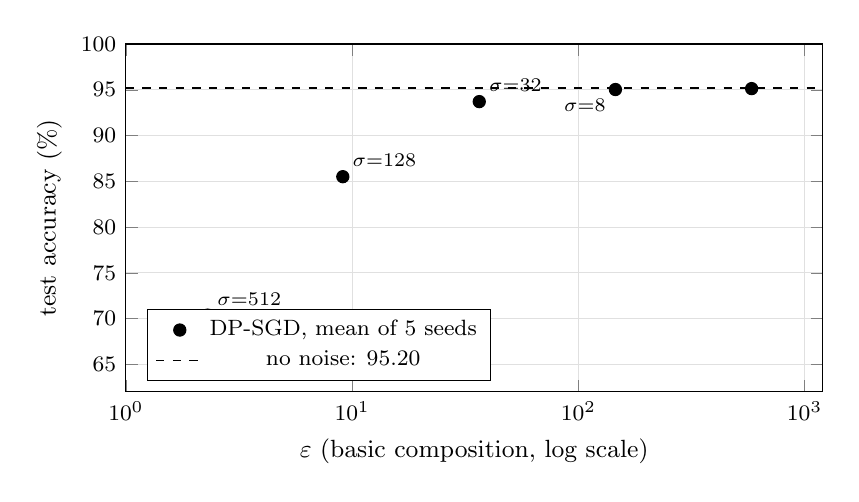
\begin{tikzpicture}
\begin{axis}[
  width=0.86\linewidth, height=6.0cm,
  xlabel={$\varepsilon$ (basic composition, log scale)},
  ylabel={test accuracy (\%)},
  xmode=log, log basis x=10,
  xmin=1, xmax=1200, ymin=62, ymax=100,
  xtick={1,10,100,1000},
  ytick={65,70,75,80,85,90,95,100},
  grid=major, grid style={black!12},
  tick label style={font=\footnotesize},
  label style={font=\small},
  legend style={font=\footnotesize, at={(0.03,0.03)}, anchor=south west},
]
\addplot[only marks, mark=*, mark size=2.2pt, black] coordinates {
  (2.3,70.39) (9.1,85.51) (36.5,93.71) (145.9,95.03) (583.7,95.13)
};
\addlegendentry{DP-SGD, mean of 5 seeds}
\addplot[black, dashed, domain=1:1200, samples=2] {95.20};
\addlegendentry{no noise: $95.20$}
\node[font=\scriptsize, anchor=south west] at (axis cs:2.3,70.39) {$\sigma{=}512$};
\node[font=\scriptsize, anchor=south west] at (axis cs:9.1,85.51) {$\sigma{=}128$};
\node[font=\scriptsize, anchor=south west] at (axis cs:36.5,93.71) {$\sigma{=}32$};
\node[font=\scriptsize, anchor=north east] at (axis cs:145.9,95.03) {$\sigma{=}8$};
\end{axis}
\end{tikzpicture}
\caption{Test accuracy against the privacy budget in the Computational lab experiment
($n=200$, $d=8$, $T=200$, $\delta=10^{-5}$, five seeds). Every point is the result of a
real execution, paired with the \texttt{eps\_basic} column in the output. The dashed line
is the accuracy without noise. The horizontal axis is logarithmic: lowering
$\varepsilon$ from $36.5$ to $2.3$ costs $23$ points of accuracy, whereas going from
$583.7$ to $145.9$ is almost free.}
\label{fig:tradeoff}
\end{figure}

\begin{figure}
\centering
\begin{tikzpicture}[scale=1.15]
\draw[->, black!60] (-1.25,0) -- (1.45,0) node[right, font=\footnotesize]
  {$\operatorname{Re}$};
\draw[->, black!60] (0,-1.1) -- (0,1.25) node[above, font=\footnotesize]
  {$\operatorname{Im}$};
\draw[black!35, dashed] (0,0) circle (0.7071);
\draw[black!55, thin] (0.7071,0) -- (0.7071,0.7071) -- (0,0.7071);
\draw[black!55, thin] (0.5,0) -- (0.5,0.5) -- (0,0.5);
\draw[->, very thick, black] (0,0) -- (0.7071,0.7071)
  node[above left, font=\footnotesize] {$a_0$};
\draw[->, very thick, black] (0,0) -- (-0.7071,0.7071);
\draw[->, thick, black!55] (0,0) -- (0.5,0.5);
\draw[->, thick, black!55] (0,0) -- (0.5,-0.5) node[below right, font=\footnotesize]
  {$a_1$};
\node[font=\scriptsize, anchor=west] at (0.75,0.16) {$\tfrac{1}{\sqrt2}=0.7071$};
\node[font=\scriptsize, anchor=north] at (0.5,-0.55) {$0.5-0.5i$};
\node[font=\scriptsize, anchor=south] at (0.5,0.56) {$0.5+0.5i$};
\draw[black!35] (0.09,0) arc (0:45:0.42);
\node[font=\scriptsize] at (0.30,0.16) {$45^\circ$};
\end{tikzpicture}
\caption{Amplitudes as arrows in the complex plane. The thick arrows are the state
$H|0\rangle$ with $a_0=a_1=1/\sqrt2$; the thin arrows are $HSH|0\rangle$ with
$S=\operatorname{diag}(1,i)$, namely $0.5+0.5i$ and $0.5-0.5i$. The modulus stays
$0.7071$, so the probability of both outcomes stays $1/2$, but the phase shifts by
$45^\circ$ in opposite directions. A measurement does not distinguish the two states; the
next gate can. The arrow coordinates are taken from the output of the Computational lab,
not drawn as an illustration.}
\label{fig:fase}
\end{figure}

Figure~\ref{fig:tradeoff} is the quantitative shape of the privacy-utility trade-off: the
curve is not linear, and the most expensive part is at the left end, in the region that is
most often praised in abstracts. Figure~\ref{fig:fase} is the geometric shape of the
sentence ``the modulus determines the probability, the phase determines the interference''.

\begin{untukdosen}
The teaching order I recommend: start from Figure~\ref{fig:tradeoff}, not from the
definition. Show that the curve has an expensive left end, then ask why. Students usually
guess ``because the noise is large'', which is true but not yet enough; what has to come
out is that the privacy budget is summed along the steps, so shrinking $\varepsilon$ per
step is paid twice, in noise and in the number of steps.

Two misconceptions almost always appear. First, students read ``$(\varepsilon,\delta)$-DP''
as ``this model is safe''. What is true is that it is a promise about the influence of one
record on the output distribution, and the model can still be completely wrong. Second,
students think the quantum phase is a decoration of notation because ``probability depends
only on the modulus''. The example $HZH|0\rangle$ breaks that in three lines.

A blackboard activity that worked in our class: ask two students to compute
$HZH|0\rangle$ and $HHH|0\rangle$ separately, then compare. Both use three gates, they
differ in only one matrix in the middle, and the results are $|1\rangle$ against
$|0\rangle$. The class is ready to go on when a student can explain why $HSH|0\rangle$
gives the same probabilities as $H|0\rangle$ but a different state.
\end{untukdosen}

\section{Summary}

\begin{ringkasan}
\begin{itemize}
  \item A model trained on personal data leaks information through three channels:
        membership, attributes, and reconstruction, and the third works from gradients.
  \item $(\varepsilon,\delta)$ differential privacy compares two output distributions for
        data that differ in one person, with the quantifier ``for every output set''. That
        quantifier is what makes the promise hold against an attacker, not merely against
        an average.
  \item The Laplace mechanism with scale $b=\Delta f/\varepsilon$ satisfies
        $(\varepsilon,0)$; its proof only compares the ratio of two densities. The Gaussian
        mechanism uses $\sigma\ge\sqrt{2\ln(1.25/\delta)}/\varepsilon$ and gives
        $\delta>0$.
  \item Basic composition adds up $\varepsilon$; advanced composition gives the better
        $\sqrt{T}$ term only when $\varepsilon$ per step is small: at $\sigma=32$ the
        results are $36.5$ versus $20.6$, whereas at $\sigma=2$ they are $583.7$ versus
        $11\,302.8$.
  \item DP-SGD clips per-example gradients at norm $C$ and then adds noise $\sigma C/B$.
        Accuracy falls from $95.20$ percent without noise to $93.71$ percent at
        $\varepsilon=36.5$ and $70.39$ percent at $\varepsilon=2.3$.
  \item Differential privacy guarantees something about individuals, not the truth of the
        model; it does not remove bias, and its utility cost can be uneven across groups.
  \item A quantum state lives in $\mathbb{C}^{2^{n}}$; a gate must be unitary because
        probability must be conserved, and measurement is the only non-unitary step. The
        output is therefore always a sample.
  \item Classical simulation needs $2^{n}$ amplitudes: $n=50$ means $16$ pebibytes. That
        fact limits imitation, but it does not prove advantage, and so far there is no
        established evidence of practical advantage for QML.
\end{itemize}
\end{ringkasan}

\section{Exercises}
\tingkat{intermediate}

\begin{latihan}
\begin{enumerate}
  \item Assess this claim: ``Our model satisfies differential privacy with
        $\varepsilon=0.5$, so no personal information can leak from it.'' State true,
        false, or not enough evidence, and name two things that must hold for the claim to
        apply.
  \item Prove that the Laplace mechanism with scale $b=\Delta f/\varepsilon$ satisfies
        $(\varepsilon,0)$ when sensitivity is measured with the $\ell_1$ norm on an output
        of dimension $d>1$. Show where the one-dimensional argument has to be replaced.
  \item Prove parallel composition: if $M_1$ works on $D_1$ and $M_2$ on $D_2$ with
        $D_1\cap D_2=\varnothing$, and each is $(\varepsilon_i,\delta_i)$, then their
        output satisfies $(\max_i\varepsilon_i,\max_i\delta_i)$.
  \item Compute $\varepsilon$ for randomized response when the probability of answering
        honestly is $p$ and the rest is answered at random with a fair coin. State
        $\varepsilon$ as a function of $p$, then determine the $p$ that gives
        $\varepsilon=2$.
  \item For a count query with $\varepsilon=0.5$ on $n=10\,000$, compute the probability
        that its absolute error exceeds $10$ people, then compare it with the same
        probability when the query is an average with $R=1$. Check both numbers by
        simulation.
  \item Compute $H\,S\,H|0\rangle$ with $S=\operatorname{diag}(1,i)$ step by step, then
        compare its probabilities with those of $H|0\rangle$. Explain why the measurement
        results are the same although the states differ, and which gate distinguishes them.
  \item For the Bell state $|\Phi^{+}\rangle$, compute the probability of the outcome $01$
        when the second qubit is measured first and the result is $0$; repeat for the
        result $1$. Explain why both answers show perfect correlation.
  \item Show that $\begin{pmatrix}1&0\\0&e^{i\varphi}\end{pmatrix}$ is unitary for every
        $\varphi$, then explain why that gate does not change probabilities in the
        computational basis but can change the result of the next gate.
  \item Compute the number of amplitudes and the memory requirement for $n=40$ and $n=60$
        qubits with $16$ bytes per amplitude. State them in sensible units, then compare
        them with the storage capacity that you have.
  \item A paper writes: ``Our circuit prepares a state with $2^{60}$ amplitudes, so it
        beats classical simulation for machine learning.'' Name three questions that must
        be answered before that sentence is accepted, and for each question state what
        kind of result would make you accept it.
\end{enumerate}

\noindent\textbf{Hints for the three hardest items.} Item 2: write the ratio of densities
as a product of per-coordinate ratios, then use $\sum_j|a_j-a'_j|\le\Delta f$. Item 3: at
every step only one of the two mechanisms can change. Item 10: whether all the amplitudes
are used, whether the output can be extracted with a number of measurements that is not
exponential, and whether there is a classical comparison on the same task and data.
\end{latihan}

\begin{untukpeneliti}
Three things in the first half are often quoted without their conditions. First, the
$(\varepsilon,\delta)$ definition here is the definition of Dwork, McSherry, Nissim, and
Smith (2006) in the form of the book by Dwork and Roth; the condition $\delta\ll 1/n$
comes from the camouflage argument for one individual, not from analytical convenience.
Second, the Gaussian bound $\sigma\ge\sqrt{2\ln(1.25/\delta)}/\varepsilon$ is loose for
small $\sigma$; the tight bound is given by the analytic Gaussian mechanism of Balle and
Wang (2018), and the difference can reach a factor of two at $\varepsilon<1$. Third, the
moments \emph{accountant} of Abadi and colleagues (2016) uses subsampling, so an
$\varepsilon$ that is reported without the subsampling rate and the number of steps cannot
be compared with other numbers.

In the second half, what is really proved is a conditional statement: complexity
separations for particular families of tasks, and the impossibility of classical
simulation for general states. What is popular but unproved is the claim that variational
circuits give an advantage on classical data. Tang (2019) and Huang, Kueng, Preskill
(2021) limit that claim from two directions: data structure can remove the speedup, and
the separations that exist depend on distributional assumptions. McClean and colleagues
(2018) show gradients that vanish exponentially in deep circuits, so variational training
has an unresolved obstacle.

The most important question is not ``is there a speedup'', but ``what kind of speedup
survives once the cost of readout, state preparation, and error correction is counted''.
Until there is an answer measured on hardware with real data, every claim of practical
advantage for QML should be read as a hypothesis.
\end{untukpeneliti}

\peta{The privacy half follows Dwork and Roth, \emph{The Algorithmic Foundations of
Differential Privacy} (chapters 2--3 and appendix A), Abadi et al., \emph{Deep Learning
with Differential Privacy} (2016) for DP-SGD, Shokri et al. (2017) for membership
inference, Dinur and Nissim (2003) for reconstruction from aggregate queries, and Zhu,
Liu, Han (2019) for reconstruction from gradients. The quantum half follows Nielsen and
Chuang, \emph{Quantum Computation and Quantum Information} (chapters 2 and 4), Cerezo et
al. (2021, 2022) for the limits of variational algorithms, Tang (2019) for
dequantization, and Huang, Kueng, Preskill (2021) for data-based separation. The
prerequisites are in Chapter 10 (SVD and orthogonality), Chapter 16 (conditional
probability), and Chapter 17 (random variables), whereas the connection to Fourier and
convolution is in Chapter 14 and Chapter 15.}
